\subsection{Extension to Other Error Models}
In many cases {FLE} cannot be properly modelled as an isotropic, independent, random variable. In the case of optical tracking systems for example \cite{736031} the errors normal to the camera plane are approximately 3 times those parallel to the camera plane. It is straightforward to implement such an anisotropic \gls{FLE} in SciKit-SurgeryFRED and test the effect on registration outcomes.

Listing 1 shows a snippet taken from the function main.getfle(). The second line defines the ratio of \gls{FLE} in three directions. By default they are all one, but in the example shown in Listing 3 the error in the x direction has been set to be three times that in the y and z directions. The results of this modification are shown in Fig. \ref{fig:anis_error}. 

\begin{pythonlisting}{\label{lis:anis} Code snippet for anisotropic {FLE}}
    fle_sd = np.random.uniform(low=0.5, high=5.0)
    fle_ratio = np.array([3.0, 1.0, 1.0], dtype=np.float64)
    anis_scale = math.sqrt(3.0 / (np.linalg.norm(fle_ratio) ** 2))
    fixed_fle = fle_ratio * fle_sd * anis_scale
\end{pythonlisting}

\begin{figure}
	\begin{center}
		\begin{subfigure}[b]{0.48\linewidth}
			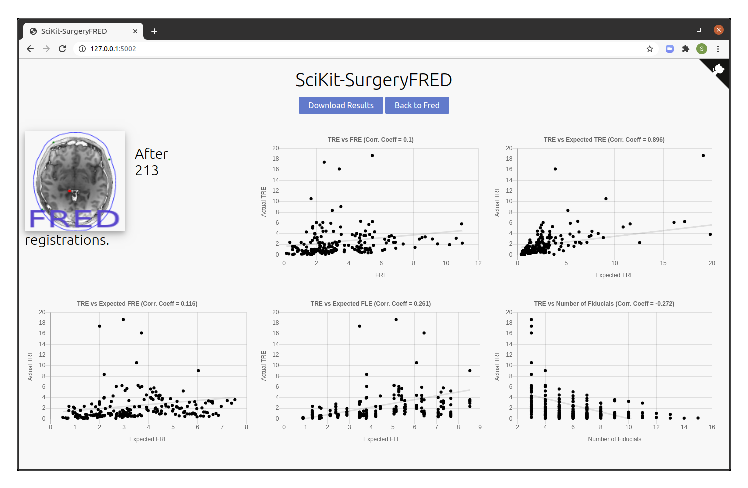
\includegraphics[width=\linewidth]{images/anisitropic_error.eps}
			\caption{\label{fig:anis_error}Anisotropic Errors}
		\end{subfigure}
		\begin{subfigure}[b]{0.48\linewidth}
			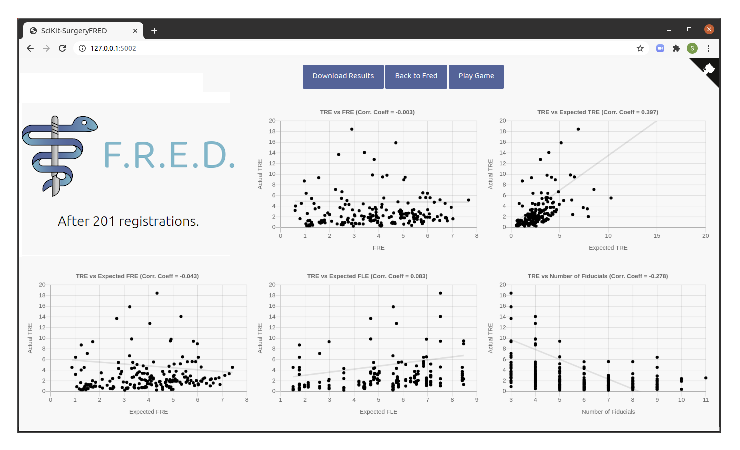
\includegraphics[width=\linewidth]{images/systematic_error.eps}
			\caption{\label{fig:sys_error}With Systematic Errors}
		\end{subfigure}
		\caption{\label{fig:other_errors}Results of over 200 registrations using an anisotropic model of {FLE} and a model with systematic {FLE}.}
	\end{center}
\end{figure}

A second significant source of error that is usually overlooked is the presence of systematic errors. For example when using a tracked pointer for fiducial localisation, and calibration error will be be added to all fiducials. Similarly some optical tracking systems can introduce a systematic error on the tracking markers \cite{6294449}. {SciKit-SurgeryFRED} allows systematic error to be added to each fiducial. Listing 4 shows 
a modification to the function init{\textunderscore}fles() in the file {static/main.js} to add a systematic error to the 
intraoperative {FLE}. Here the error is an isotropic uniform random variable, in the range -0.5 to 0.5. This error will be applied to all fiducial markers for a given registration. The results of this modification are shown in Fig. \ref{fig:sys_error}.

\begin{javalisting}{Java to generate independent FLE}
	preOpSysError = [0.0, 0.0, 0.0];
        intraOpSysError = [1.0 * (Math.random()-0.5), 
		1.0 * (Math.random()-0.5), 
		1.0 * (Math.random()-0.5)];
\end{javalisting}

